% Copyright 2020 by Robert Hildebrand
%This work is licensed under a
%Creative Commons Attribution-ShareAlike 4.0 International License (CC BY-SA 4.0)
%See http://creativecommons.org/licenses/by-sa/4.0/

\section{Polyhedra}

\subsection{Convex Hull}

\begin{verbatim}
[[0.78913 0.2673 ]
 [0.5462  0.79165]
 [0.29012 0.53835]
 [0.97705 0.57501]
 [0.32814 0.99928]
 [0.87902 0.53254]
 [0.36117 0.57705]
 [0.48521 0.85347]
 [0.75269 0.24459]
 [0.81315 0.47965]
 [0.60529 0.84873]
 [0.64951 0.57425]
 [0.57901 0.27927]
 [0.53027 0.83896]
 [0.85029 0.11324]
 [0.19383 0.7854 ]
 [0.07971 0.80899]
 [0.4783  0.41661]
 [0.88042 0.37067]
 [0.25369 0.00183]
 [0.73571 0.56145]
 [0.29421 0.32336]
 [0.11878 0.76099]
 [0.2648  0.40023]
 [0.31803 0.57827]]
Single polytope 
  [[ 0.96433 -0.26471] |    [[ 0.78998]
   [-0.60809  0.79387] |     [ 0.59376]
   [ 0.18357 -0.98301] x <=  [ 0.04477]
   [-0.97755 -0.2107 ] |     [-0.24838]
   [ 0.5929   0.80528] |     [ 1.04234]
   [ 0.47734  0.87872]]|     [ 1.03472]]
\end{verbatim}

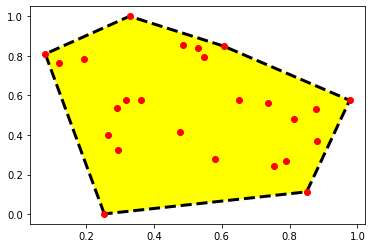
\includegraphics[scale = 0.5]{convex-hull-random}


